%
% This template has been created by:
% Pascal Bercher, pascal.bercher@anu.edu.au
%
% This is version 1.01 (13. Sep 2022)
%
% version history:
% - 1.00 (3. Dec 2021)  - first version that deserves a version number! :)
% - 1.01 (13. Sep 2022) - fixed wrong TOC link to Bibliography
%
% Make sure to use the newest version available on git!
%
% I was too lazy to put it under a specific license, but you are still free to use and alter it.
% But since I put a *lot* of effort (and experience)

\documentclass[a4paper,twoside,cleardoublepage=plain,bibliography=totoc]{scrbook}

\usepackage[a4paper]{geometry}                    % used for defining the title page

\usepackage{xurl}                                 % allows long URLs to break at any position
\usepackage[backref=page]{hyperref}               % defines style of references / links
\hypersetup{
linktocpage,                                      % in the table of contents, the numbers serve as links, not the entries
colorlinks  = true,                               % the items are colored instead of colored boxes around them
urlcolor    = cyan,
linkcolor   = red,
citecolor   = blue
}
% the following makes back references more appealing.
% Taken from: https://tex.stackexchange.com/questions/183702/formatting-back-references-in-bibliography-bibtex
\renewcommand*{\backref}[1]{}
\renewcommand*{\backrefalt}[4]{[%
\ifcase #1 Not cited.%
  \or Cited on page~#2.%
  \else Cited on pages #2.%
\fi]}




\usepackage{datetime}                             % to be able to print month & year on title page
  \newdateformat{monthonly}{\monthname[\THEMONTH]}
\usepackage{amssymb,amsthm,amsmath}               % standard math packages; often used
\usepackage{graphicx}                             % allows including graphics
\usepackage{natbib}                               % a specific citation style
\usepackage{floatrow}                             % allows to place a caption next to a figure
  \floatsetup[table]{capposition=top}             %  forces table captions to appear on top.
\usepackage{booktabs}                             % for tables that actually look nice!
\usepackage{paralist}                             % provides compactitem, a more compact itemize
\usepackage{titlesec}                             % used to add those horizontal lines around chapter package; see defs below.
\usepackage[standardsections]{scrhack}            %  fixes an error causes by loading titlesec for class scrbook
\usepackage{parskip}                              % when this is included, no indentations are used for new paragraphs,
                                                  % and instead paragraphs are separated by a small distance between them


% [requires titlesec]
% Surrounds all chapter titles by lines,
\titleformat{\chapter}[display]
{\bfseries\huge}
{\filleft\Large\chaptertitlename~\thechapter}
{3ex}
{\titlerule\vspace{1.5ex}\filright}
[\vspace{1ex}\titlerule]

% fixes a compilation errror that otherwise occurs in combination with scrbook
% see https://tex.stackexchange.com/questions/625083/adding-horizontal-line-before-and-after-chapter-heading-in-scrbook
% \titleformat{\section}
%  {\normalfont\Large\bfseries}{\thesection}{1em}{}
% \titleformat{\subsection}
%  {\normalfont\large\bfseries}{\thesubsection}{1em}{}
% \titleformat{\subsubsection}
%  {\normalfont\normalsize\bfseries}{\thesubsubsection}{1em}{}
 

 

% Set your individual data for the title page in the configuration file
% AND DONT SCREW UP THIS DATA! You should know, for example, whether it's
% an Honours thesis or not, or in which semester it is running.

% well, the title!
\title{%
  Logic (COURSE TITLE)\\
  \emph{Chapter:} \textbf{CHAPTER TITLE}%        MUST BE UPDATED FOR EACH LECTURE
}

% well, the date!                                SHOULD BE SET MANUALLY TO THE DATE OF THE RESP. LECTURE
\date{\today} %                                  

% well, the author!                              UPDATE!
\newcommand{\FirstLecturer}  {PERSON 1}           % \author is overwritten by the style,
\newcommand{\SecondLecturer} {PERSON 2}           % so don't specify it!

% well, your affiliation!                        UPDATE!
\newcommand{\GroupFirstLecturer}  {GROUP 1}
\newcommand{\GroupSecondLecturer} {GROUP 2}
\institute{THE UNIVERSITY/COLLEGE}
                             % to specify data used in the title page

% define your own macros here

\newcommand{\Eff} {\ensuremath{\mathit{eff}}}  % example command without arguments
\newcommand{\Pre} {\ensuremath{\mathit{pre}}}  % (again)

% Note that you can easily specify arguments:
% \newcommand{\someMacro}[2] {Argument 1: #1, Argument 2: #2} % example command with two arguments
% you use it via \someMacro{Hello}{World!}


% the following commands are being provided by the amsthm package
% the first parameter states the new environmet's name that can be
% used (due to this definition here) and the second the name that
% will appear in the PDF document
\theoremstyle{definition}
\newtheorem{definition}{Definition}   % well, a formal definition!
\theoremstyle{plain}
\newtheorem{prop}{Proposition} % like a theorem, but less important or evolved
\newtheorem{lem}{Lemma}        % used within a proof of a theorem
\newtheorem{thm}{Theorem}      % well, a theorem! :) important and evolved
\newtheorem{cor}{Corollary}    % basically either a proposition or theorem,
                               %  but one that follows from another theorem.
% There's a lot you can configure about the appearance. If interested,
% open the manual of amsthm or google for tutorials etc. on that package

% the following add a symbol to the definition environment to make it more
% clear when a definition ends (as there is no difference in fonts!). From:
% https://tex.stackexchange.com/questions/226334/change-a-amsthm-theorem-ending
\newcommand{\xqed}[1]{%
    \leavevmode\unskip\penalty9999 \hbox{}\nobreak\hfill
    \quad\hbox{\ensuremath{#1}}}
\newcommand{\Endofdef}{\xqed{\blacksquare}}
\newenvironment{defn}[1]{%
    \begin{definition}#1}{%
    \Endofdef\end{definition}%
}
                                    % define all your macros here


\begin{document}

\pagenumbering{roman}

%
% This document contains two different definitions of the title page
% which one is chosen is defined in the file configutation.tex
%


% only the title page is centered; all other pages are aligned according to books
\newgeometry{left=2.5cm,right=2.5cm,top=2.5cm}
\thispagestyle{empty}

\newdateformat{monthyeardate}{%
  \monthname[\THEMONTH] \THEYEAR}


\ifStandardTitle % the first style is defined now

\noindent
\begin{minipage}[t]{6cm}%
{\footnotesize%
\raisebox{-\height}{{\bfseries The Australian National University}} \\
~2600 ACT~\textbar~Canberra~\textbar~Australia}
\end{minipage}%
\hfill%
\begin{minipage}[b]{10cm}%
\hfill\raisebox{-\height}{
\includegraphics[height=2 cm]{figures/ANU-logos/ANU_Primary_Horizontal_Black.jpg}}
\end{minipage}


\ \\[2em]
\phantom{x} \hfill
\begin{minipage}{58.75 mm}
\raggedright
\bfseries \School\\[.5em]
\mdseries%
\noindent\College
\end{minipage}\\[6 em]
\hfill

\noindent
\parbox{140mm}{\sffamily \bfseries \Huge %
\ProjectTitle%
}\\[.75 em]
{--- \ProjectPoints{} pt \ifHonoursThesis Honours \else research \fi project (\Semester{} \Year)}\\[3 em]


\ifHonoursThesis%
A thesis submitted for the degree\\
\emph{\Degree}\\[3 em]
\else%
A report submitted for the course\\
\emph{\CourseCode, \CourseName}\\[3 em]
\fi




\noindent
{\footnotesize \textbf{By:}}\\
\AuthorName\\[2em]



\noindent
{\footnotesize \bfseries Supervisor\ifTwoSupervisors{}s\fi:}\\
{\footnotesize \FirstSupervisor%
\ifTwoSupervisors\\\SecondSupervisor\fi}\\[2 em]
\vfill
{\footnotesize \monthyeardate\today}



\else % the alternative design of the title page



\begin{center}
\ \\[1em]
{\bfseries \Huge \ProjectTitle}\\[4em]
%
\ifHonoursThesis%
\Large{A thesis submitted for the degree}\\
\Large{\emph{\Degree}}\\[.5em]
{\ProjectPoints{} pt Honours project, \Semester{} \Year}
\else%
\Large{A report submitted for the course}\\
\Large{\emph{\CourseCode, \CourseName}}\\[.5em]
{\ProjectPoints{} pt research project, \Semester{} \Year}
\fi
%
\ \\[4em]
{\footnotesize \textbf By:}\\
\textbf{\AuthorName}\\[3em]
%
{\bfseries Supervisor\ifTwoSupervisors{}s\fi:}\\
{\FirstSupervisor%
\ifTwoSupervisors\\\SecondSupervisor\fi}\\[6em]
%

\includegraphics[height=2.5cm]{figures/ANU-logos/ANU_Primary_Horizontal_Black.jpg}\ \\[3em]
%
{\bfseries \School}\\
{\mdseries \College}\\
The Australian National University
%
\vfill
\normalsize{\monthyeardate\today}
\end{center}



\fi


\restoregeometry
                               % define your title page
{\sffamily\bfseries\Large Declaration:}\\

I declare that this work:\\

\begin{itemize}
  \item upholds the principles of academic integrity, as defined in the \href{https://www.anu.edu.au/about/governance/legislation}{University Academic Misconduct Rules};
  \item is original, except where collaboration (for example group work) has been authorised in writing by the course convener in the class summary and/or Wattle site;
  \item is produced for the purposes of this assessment task and has not been submitted for assessment in any other context, except where authorised in writing by the course convener;
  \item gives appropriate acknowledgement of the ideas, scholarship and intellectual property of others insofar as these have been used;
  \item in no part involves copying, cheating, collusion, fabrication, plagiarism or recycling.
\end{itemize}


\vspace{1 cm}
\hfill \monthname, \AuthorName
\newpage


% The current requirements can be found on:
% https://policies.anu.edu.au/ppl/document/ANUP_004603  (section 18) -- date: 9.2.2022
                             % includes the declaration of authorship
\chapter*{Acknowledgements}

If you wish to do so, you can include some Acknowledgements here. If you don't want to, just comment out the line where this file is included.

There is absolutely no need to write an Acknowledgement section, so only do so when you want to -- i.e., if there's somebody you really want to thank (for example if you received extraordinary supervision). The more important the work, the more likely that an Acknowledgement section doesn't look off. In a 24 pt.\ Honours thesis it would for example look more reasonable than for a 6 pt.\ project report.\\

\textbf{Unrelated to the Acknowledgements, but important:}

\emph{Note that there exist two different title page designs.} You may choose the one that you find more appealing. Just use the configuration file to select this style. There, you also have to put in all the other information about this report like your name, the kind of report (Honours vs non-Honours) and so on.
                        % optional acknowledgements
\chapter*{Abstract}

An abstract is a very short summary (around 15 lines) of your entire work (that doesn't use citations by convention). There are plenty of examples you can take a look at -- simply take a look at some papers published at top-tier venues, e.g., by your supervisor.
                                % your abstract

% table of contents (nothing to do for you)
\renewcommand{\contentsname}{Table of Contents}   % would otherwise just be "Contents",
\cleardoublepage\tableofcontents\cleardoublepage  % which might sound less nice
\pagenumbering{arabic}

% actual report content
\chapter{Introduction}

The introduction serves two purposes: \hfill (Not necessarily in this order.)
\begin{compactenum}
  \item To give a high-level \emph{introduction} into the research area and\label{enum:intro:introduction}
  \item to \emph{motivate} your research done within it.\label{enum:intro:motivation}
\end{compactenum}

Point \ref{enum:intro:introduction} is important because you should not assume any technical background in the specific subject matter of your work. Provide a high-level introduction, but avoid technical definitions unless they are used as an easy-to-understand example that doesn't require prior knowledge. The rule of thumb is that you can assume a very basic understanding of the respective (more general) research area, like computer science, engineering, mathematics, and so on -- based on the audience for which the work is conducted. What such an accurate level of abstraction/presentation is might depend on the specific topic of your work. Also consult your supervisor(s) for their opinion(s) and preferences. 

Point \ref{enum:intro:motivation} should make clear why the investigated research question is worth being investigated -- why is it relevant and important? This is the part where you should make the readers look forward reading your work! Make them interested and passionate!

Be specific about the precise contributions that your work actually does and list them in the text (preferably in a separate paragraph; depending on the number of contributions and how well they can be separated you could also provide them in a bullet point list).

An introduction is usually between 1 and 3 pages. You can also get some inspiration from papers published at top-tier conferences, although they are of course \emph{much} shorter due to space constraints.

Some people prefer ending the introduction with a paragraph that gives an overview of the following chapters. However, this is more usual for scientific papers (published at conferences or in journals) but not in project/thesis reports since they have a table of contents anyway. You are still free to add one if you prefer.
                            % introduction
\chapter{Background}\label{chap:background}

This section should explain all the technical background that is important for being able to read your report. Recall that your report must be completely self-contained, so you should only assume ``mathematical understanding'', but no specific knowledge. All such knowledge should be provided here, e.g., the formalization and vocabulary of the research areas in which your work resides.

Note that this is not the same as reviewing related work. Related work puts the work done/described in your report into context of other (mostly recent) work that's done by others. In contrast the current chapter is not so much about what work others have done, and more about the formalization (and possibly standard techniques) that you require to describe your contributions (but since you probably didn't come up with these formalizations, you of course still need to cite the respective authors).

Please make use of sections and subsections as it's reasonable to better structure this (or any) chapter.
                              % background/framework
\chapter{Related Work}\label{chap:relatedWork}

This chapter reviews the work that is most related to the research questions investigated by you in this work. Please note that there are various options on \emph{where} you include it.

\begin{itemize}
  \item You could include it \emph{here} (i.e., where you see it right now in the template). Since it's after the formal definitions (Chapter~\ref{chap:background}), you can explain what the other works have done on some level of detail, yet you need to keep in mind that you did not yet explain your own contributions (except abstractly in the abstract), which slightly limits the level of technical detail on which you can compare these approaches here.
  
  \item You could also make it a subsection of Chapter~\ref{chap:background}. This choice might also depend on the length of this chapter. Is it worth its own full chapter?

  \item Alternatively, you might include this chapter after the main part of your report, i.e., right before Chapter~\ref{chap:conclusion}. When you do this, you can go into more technical detail since the readers will have read your entire work, so they know exactly what you've done and you can therefore discuss differences (like pros/cons etc.) in more detail.

  \item When you take a look at scientific papers (preferably at top-tier venues), you might notice that not every single paper has a related work section. This is because in principle related works might also be addressed/positioned in the introduction or in the main part of the work. But since this is not a ``standardized scientific publication'', it is very strongly advised that you devote its own section to related work as done in this template.
\end{itemize}

If you prefer any of the latter two options, discuss this with your supervisor(s).
                             % related work
\chapter{Reasonable Title for Main Content}\label{chap:content}

This chapter holds your actual contributions. Depending on what you did in your project you might either use just one chapter describing your contributions or you use multiple ones -- think about this and consult your supervisor(s). Apart from the empirical evaluation (if there is any) -- is the main part of your work and thus the core of this document. In any case, give this chapter/these chapters a reasonable name\footnote{You may also rename the tex filename if you wish.} and explain clearly what you have done and how it builds upon or extends the closeliest related work.

The following sections give additional advice that is specifically tailored to students who are new to either \LaTeX{} or scientific writing.



\section{General Advice}

\begin{itemize}
 \item \textbf{Start early.} Writing a report is hard and takes time. More than you think. \emph{Hofstadter's Law:} ``It always takes longer than you expect, even when you take into account Hofstadter's Law.'' -- \emph{So start early!}
 \item \textbf{Read and check your work!} First of all, please use a spellchecker! Each \LaTeX{} editor should support this, so please always turn it on. Secondly: Read your work \emph{carefully} and \emph{multiple times} before showing it to your supervisor. Your supervisor is surely happy to help you -- that's her/his/their job! But you will benefit from investing your time: Assume that her/his/their time investment is always the same $n$ -- so the more of this doesn't have to be invested for errors you could solve yourself, the more time can be invested for more important advice.
 \item \textbf{Involve your supervisor!} Don't be afraid to reach out to your supervisor(s)! She/he (they) is (are) literally being paid to supervise you and help you succeed! :) So make sure you get what you need to be successful, don't hold back.
\end{itemize}


\pagebreak %
\section{Building the PDF}

\begin{itemize}
  \item \textbf{Latexmk:} This very useful commandline tool works on all standard operating systems: Linux, macOS, and Windows. The installation overhead is minimal, and on Linux you probably have \emph{everything} already installed! Check it out here: \url{https://mg.readthedocs.io/latexmk.html} -- this is the preferred option since it's the most convenient and takes the least time to run, i.e., compile.
  \item \textbf{makefile:} If you use Linux (and potentially macOS) you can use the provided makefile, which features five different functions.
  \begin{itemize}
    \item Executing ``make'' (i.e., executing that command in the project's folder) is the same as executing ``make mk''. This is nothing else than a shortcut for the Latexmk program, but with the required parameters. This is the preferred way since Latexmk ``magically'' knows what it has to do, i.e., what to compile and how often.
    \item ``make mkonline'' is an extension of the above: it runs Latexmk in an online mode that compiles again after every single change that is saved; so you always see the newest version automatically without having to re-compile.
    \item ``make all'' will compile the document multiple times (1 times bibtex, 4 times pdflatex). This makes sure that all references like links to page numbers and figures work correctly, and that all citations are correctly processed. Note that this is not required if you use any of the above options, as those are basically the ``state of the art'' and do the minimal amount of required work.
    \item You may also call the script via ``make quick'', which compiles exactly once. This is much quicker than the last, but may not process all references correctly. Again, Latexmk is the preferred option. It even doesn't do anything if that's not required.
    \item With ``make clear'' you can conveniently delete all temporary files. This is sometimes required if compilation fails (e.g., when you create wrong bibtex entries, which may be caused by non-supported symbols or commands).
  \end{itemize}  
\end{itemize}




% the optional argument appears in the table of contents (TOC). Use that in case the *actual* title is too long 
% and would therefore not look well.
\section[Technical Advice for Writing Your Report]{Technical Advice (\LaTeX{} etc.), Rules for Writing Reports, and Scientific Advice}

\begin{itemize}
  \item \textbf{Watch Your Dots:} You need to ``escape'' all blanks following a dot that is not ending a sentence. E.g., the sentence ``This is 6 pt.\ project.''\ needs to be coded ``\verb!This is 6 pt.\ project.!'' as otherwise it looks as follows: ``This is 6 pt. project.''\ -- you see that in here the spacing after ``pt.''\ is wrong (i.e., way too large). This is because \LaTeX{} interprets each dot (with a following space) as one that ends a sentence -- after which more space is allocated. An escaped space in contrast produces a fixed space that doesn't get stretched. (Fun fact: when (mechanical) typewriters were still a thing, authors were hitting the space twice after each ``sentence-ending dot'' to produce exactly the behavior that \LaTeX{} does automatically.)
  % for those who *really* want to do everything right: When you look at the code above you see that the escaping is used in even more situations than claimed in the PDF. It is also used after closing quotation marks that have a preceding dot. The reason is that in this situation 
  
  \item \textbf{Headlines/Titles:}
  \begin{itemize}
    \item Titles (chapters, sections, subsections) are capitalized according to specific rules. Basically everything is written capitalized except of some specific words (in, on, the, $\dots$). You can search for capitalization rules and even tools, which you might find useful to be consistent.
    \item Also note that -- purely due to aesthetical reasons -- you should:
      \begin{itemize}
        \item Always have at least one line of ``glue text'' between the chapter title and the first section, i.e., anything that briefly introduces what comes next.
        \item Never use exactly one section. If you use sections, there should be at least two -- because otherwise it's just pointless; you could (if you had just one section) just eliminate it as otherwise the chapter title should then already reflect the content.
      \end{itemize}
  \end{itemize}


  \item \textbf{Appearance:} Don't forget that your work isn't parsed by a robot, but read by a human being. So make it pleasant for them, i.e., optically pleasing. Some examples:
  \begin{itemize}
    \item \emph{Page and Line Breaks:} If some headline ends up at the end of a page, that might look ugly. Consider adding \verb!\pagebreak! right before it to force placing it on the next page. That will likely look much nicer. In some rare cases you might want to do the same on a per-line basis, where you can use the \verb!\linebreak! command to enforce a linebreak at that position. In the same context the command \verb!\mbox{}! might be useful, which prevents a linebreak of the word(s) specified as argument.
    \item \emph{Big Gaps in the Document:} Make sure that there are no huge gaps in the middle of your report/text, e.g.:
    \begin{itemize}
      \item For example, make sure that a chapter doesn't end with a single line on a new page, that's just ugly and thus careless. The same applies for the table of contents: If it happens to have so many entries (sections/subsections etc.) that it jumps to a next page just because of one or two lines/entries, then just search (e.g., using stackoverflow) how to reduce the space between the lines so that it fits. Show some effort.
      \item Also make sure that when including figures or tables that there is no huge gap before them, that may happen depending on their size.
    \end{itemize}
    \item \emph{Respect Boundaries!} Another thing that's often done ``wrong'' regarding appearance is having expressions (mostly formulae) going over the allowed border. That is ugly and careless, so rephrase to prevent that. (That would even be strictly forbidden in the context of publishing a paper.)
  \end{itemize}
  Do all of this \emph{briefly before you hand in}, as all that depends on your final layout. Adding, changing, and removing text will of course change the appearance, so do all this in a very final step.
  
  
  \item \textbf{Appearance of Mathematical Expressions and Algorithms:} This is \emph{not} a \LaTeX{} tutorial, so only frequent beginner's errors are being mentioned and abstract advice is provided. For an introduction to \LaTeX{} see the last list entry.
  \begin{itemize}
    
    \item \emph{General advice:} If you are new to \LaTeX{} and need to write down a lot of formulae, theorems, or algorithms etc., spend a few minutes to at least scroll through the manuals of the respective standard packages -- this will already show you examples of the appearance of what you can do. Just search for the manuals for \verb!amsmath! (for equations), \verb!amsthm! (for theorems/propositions), and \verb!algorithm2e! (for algorithms).
    
    \item \emph{Variable names:} Very often, variable names will not be single letters, but \emph{words}, such as \emph{pre} for precondition or \emph{eff} for \emph{effects}. Since variables are usually used in math mode, there's the temptation to just write them in math mode. For example, one might write \verb!$\langle pre,eff\rangle$!, resulting into ``$\langle pre,eff\rangle$''. You hopefully see that this looks incredibly ugly -- because \LaTeX{} sets the text incorrectly. Instead, you should put it into math italics. To save you effort, you should define a new macro:
    \begin{center}
      \verb!\newcommand{\Pre} {\ensuremath{\mathit{pre}}}!\\
      \verb!\newcommand{\Eff} {\ensuremath{\mathit{eff}}}!
    \end{center}

    With this you can now simply write \verb!$\langle \Pre,\Eff\rangle$!, which now results into $\langle \Pre,\Eff\rangle$, which looks exactly as it should. Do this for \emph{all} your variables to make sure they look nice. (This template includes the file macros.tex, which you can use for all your macros.)
  \end{itemize}

  
  % the figures are put in here so that it can be moved around in the document more easily
  % (since this way it's one line to move, otherwise it might be a large block of code)
  \begin{figure}[th!]
  
\includegraphics[width=4.5cm]{figures/pexels-ann-h-3095771.jpg}
  \caption{A caption for the illustrated graphic \citep{pictureSource}. It's made long on purpose so that you can see that it simply doesn't look good that the caption is below -- since there is now a lot a free/unused space. It would have been a better choice to place the caption next to it, which you can see in Figure~\ref{fig:graphicCaptionAside}.\label{fig:graphicCaptionBelow}}
\end{figure}%
%
\begin{figure}[bh!]
  \floatbox[{\capbeside\thisfloatsetup{capbesideposition={left,top},capbesidewidth=10cm}}]{figure}[\FBwidth]
  {\caption{Captions should not explain/interpret graphics, but enable the reader to read it. Further interpretations and conclusions should be in the text only. For this graphic the following caption might be appropriate: ``Motivational expressions written and pinned on a wooden fence~\citep{pictureSource}.''\ \\[1em]
  %
  Also note how in this case the caption should be on the left (and not below the graphic as in Figure~\ref{fig:graphicCaptionBelow}) as otherwise there would be a lot of free/unused space. The code for this is a bit more complicated, but now you can simply change it, so it should be fine... :) \label{fig:graphicCaptionAside}}}
  {
\includegraphics[width=4.5cm]{figures/pexels-ann-h-3095771.jpg}}
\end{figure}

  
  
  \item \textbf{Graphics/Pictures:}
  \begin{itemize}
    \item The most important thing to know about graphics is that they ``float''. That is, \LaTeX{} decides where they should be placed, not you. You can of course influence that a bit (e.g., by the arguments for the figure environment, cf.~\url{https://tex.stackexchange.com/questions/39017/how-to-influence-the-position-of-float-environments-like-figure-and-table-in-lat}), depending on where you put the source code that includes the graphics, but \LaTeX{} will have the final word on where \emph{exactly} it will appear. Still, please make sure that your graphics appear at reasonable places so that reading the document remains being a pleasure. Anyway, that means that you will have to reference/cite each graphic. Thus, the reader will take a look at a graphic (i.e., figure) exactly when you reference it in the text, not when it's ``being seen''. (This also means that graphics/figures that are not referenced could and should be deleted from your work.)
    \item In Figure~\ref{fig:graphicCaptionBelow} you see an example figure with its caption below -- which looks very ugly. Do that if the graphic is centered and wide enough. In contrast, Figure~\ref{fig:graphicCaptionAside} provides the caption next to the figure -- which in this case looks quite good since the graphic is portrait rather than landscape, i.e., now there are no white/lost spaces.
  \end{itemize}

  
  \item \textbf{Colored Links:} By default you will see that all hyperlinks (e.g., to figures like Figure \ref{fig:graphicCaptionAside}, citations like by \cite{Smith2021Wubalubadubdub}, etc.) are colored. Personally, I (the author of this template) find that easier to read in the PDF than the alternative. The alternative is that hyperlinks are indicated by colored boxes that surround them (where the text itself remains black). You can choose between the two by the setting the option \verb!colorlinks = true! or \verb!colorlinks = false! in the hyperref definitions (where \verb!true! colors the words, whereas \verb!false! produces the box). Note a major difference between the two: The box is an annotation, so it's not visible when printing. If the text itself is colored then that's an actual text color, so it will appear as you see it in the PDF also in the printout. You can of course also change the colors.

  
  \item \textbf{Tables:} Standard \LaTeX{} tables don't look particularly pleasing. Thus, it's generally recommended to use the \verb!booktabs! package, which was designed to produce aesthetically pleasing tables. Table~\ref{tab:meatPrices} provides an example, taken from the official manual (slightly adapted). One of the most important rules: Do not use vertical lines. Note that the table caption appears on top. This is set on purpose to align with several publishers, who demand that captions for tables are \emph{above} tables, whereas those for figures (i.e., everything else: graphics, plots etc.)\ are \emph{below}.

  \begin{table}[h] % the "h" means "here", so using that places it at a nicer position
    \begin{tabular}{llr}
      \toprule
      \multicolumn{2}{c}{\textbf{Item}} \\
      \cmidrule(r){1-2}
      \textbf{Animal} & \textbf{Description} & \textbf{Price} (\$)\\
      \midrule
      Gnat            & per gram             & 13.65      \\
                      & each                 & 0.01       \\
      Gnu             & stuffed              & 92.50      \\
      Emu             & stuffed              & 33.33      \\
      Armadillo       & frozen               & 8.99       \\
      \bottomrule
    \end{tabular}
  \caption{This table lists prices for different kinds of animal meat.\label{tab:meatPrices}}
  \end{table}

  
  \item \textbf{Bibliography:} There are various points that you should consider when you add a publication into your bibtex file. The first basic rule is: \textbf{\emph{never blindly copy some bibtex entry from the internet}} -- most of them are of very poor quality. Instead, double-check each entry by hand via trustworthy sources, such as DBLP (\url{https://dblp.org/}), the publisher's webpage, or the websites by the authors. For each entry, consider the following:
  \begin{itemize}
    \item \emph{Correctness:} Is the type correct? For example, papers published in conferences should be ``inproceedings'', papers published in journals are ``article''. These are often wrong when using non-trustworthy internet sources. Also check the content like year, page numbers, etc.
    \item \emph{Completeness:} Make sure that each entry contains all fields that are required (like authors, title, booktitle etc.) but also those that are ``usually specified''. The latter is hard for a beginner, so this is the recommendation: Also provide page numbers, publisher, year.
    \item \emph{Consistency:} Make sure that the various entries are consistent to each other. For example, conference papers usually use acronyms. Make sure to either always add the respective acronym (preferred) or never. If you add it, add it always in the same way. E.g., don't add ``..., IJCAI-12'', ``... (IJCAI-12)'',\linebreak ``... (IJCAI '13)'', ``... (IJCAI 2015)'' -- use always the the systematicity. Likewise with the conference titles. For example, do not write ``Proceedings'' for one but ``Proc.'' for another. Stay consistent.
  \end{itemize}
  
  
  \item \textbf{Citing Papers:} In most cases, you place a citation right behind the respective proposition that you want to back up. Let's assume that the next citation backs up the sentence that you currently read \citep{Smith2021Wubalubadubdub}, it was thus plausible to put it exactly there -- and not at another position of this sentence. To use this kind of citation (that you put behind the respective proposition), you use the command \verb!citep{}!. However, if for some reason you need or wish to use the paper \emph{explicitly} within your sentence, then refer to its \emph{authors} (not the paper) using the \verb!cite{}! command. For example, I can claim that the work by \cite{Smith2021Wubalubadubdub} will be quite funny once it will have been done! This is just nicer than claiming that the work ``described in \citep{Smith2021Wubalubadubdub}'' will be influential. The reason is again consistency, because normally citations like the very first one (where everything is contained by parentheses, not just the year) are not objects of the sentence. So using them sometimes as objects and sometimes not would be inconsistent.

  In addition to the commands \verb!citep{}! and \verb!cite{}!, \verb!\citeauthor{}! is sometimes useful. This just lists the author(s), but without the year. I.e., it's an alternative  to \verb!cite{}! that you should use when you want to mention the authors whereas you used similar citations before so that there is just no need to add the year again.
  
  Also note that you can easily cite multiple works with one command as shown in (the code of) this sentence \citep{Cooper2015SuperfluidVacuumTheory,Smith2021Wubalubadubdub}.

  
  \item \textbf{\LaTeX{} Issues?} One of the best sources for solving \LaTeX{} issues is \url{https://stackoverflow.com/}. In case your document doesn't compile, check out the log file and search for ``error'', often that points towards the problem quickly. I (the author of the template) recommend to use the ``online version'' of Latexmk (reminder: which you can execute by simply executing ``make mkonline''), because then the document recompiles every single time you save (and showing any error message in the terminal) -- so you should find your coding errors instantly since you know what you have done when the error was introduced. If the online mode fails, fix the error and enter a large X, compilation will then continue.

  You might also want to take a look at a well-known \LaTeX{} introduction \citep{Oetiker2021LatexIntroduction}, which in the current version -- according to \citeauthor{Oetiker2021LatexIntroduction} -- takes ``only'' a bit more than two hours to work through.

  \item \textbf{Definitions and Theorems.} In theses or project reports in computer science or engineering you are bound to have definitions. It is at your discretion whether you provide some definition purely ``in-text'' or whether you make aware of it more prominently by using a definition environment. It's sometimes hard to judge what should go into the former and what should to into the latter, in particular for beginners. In my experience, beginners put too much into formal definitions, because they think everything is important. :) If in doubt, reach out to your supervisor early, he/she will know! My personal stands on that is that you should only use a formal definition environment if at least one of the following criteria is satisfied: The definition will be referenced/mentioned later on again (rather than just ``using'' it), or the defined concept is simply very ``important'' or ``central'' (again, it might be hard for you to judge what that means, so reach out to your supervisor if in doubt).

  For a sake of providing an example for how it looks in this (PDF) document, but also so that you can see how to use the \LaTeX{} commands, I borrow from some simple concepts of AI planning.

  \begin{quote}In planning, we talk about \emph{states}. States are subsets of \emph{propositions} or \emph{facts} taken from a finite set of available fact $F$ that can used to describe our system/world. Thus, states $s\subseteq F$ are those facts which are true in the respective current world state $s$. $\dots$ The finite set of actions $A$ is given by $\dots$ A given sequence of actions $\bar{a}=a_1\dots a_n$ applied to a state $s\in 2^F$ leads to a state $s'\in 2^F$ if and only if $\dots$\end{quote}

  Note that all concepts described here are of course quite foundational, but none of them seems to be ``evolved enough'' to warrant putting them into a formal definition environment. It is much more natural so simply introduce these (formal!) definitions within a text. Some of these components introduced above together form the components of a \emph{planning problem}, which is essentially the main concept in AI planning. If thus deserves its own \emph{formal} definition, which will appear as follows:

  \begin{defn}[Planning Problem]\label{def:planningProblem}A \emph{planning problem} is a 4-tuple $\langle F, A, s_o, G\rangle$ consisting of:
  \begin{compactitem}
    \item $F$, a finite set of \emph{facts}
    \item $A\subseteq F\times F\times F$, a finite set of \emph{actions},
    \item $s_0\in 2^F$, the \emph{initial state},
    \item $G\subseteq F$, the \emph{goal description}.
  \end{compactitem}
  Some (fake) text that's still part of the definition.
  \end{defn}

  You may see that sometimes it's hard to recognize where a definition ends and where the normal thesis/report text continues. For this reason I added a black box at the end of all definitions. If you don't like that use the ``definition'' environment rather than this ``defn'' environment. Also note that your definition gets numbered! This for example is Def.~\ref{def:planningProblem}. You can configure how definition numbers are shown, e.g., whether they are simply consecutive (as it's right now) or whether these numbers are prepended by the chapter/section number to make finding them easier. Just use the \textsc{amsthm}'s package manual and stackoverflow to find out!

  Finally, but \emph{really} important for any beginner: Note that formal definitions can \emph{never} contain explanations. They only contain plain boring definitions themselves (as above). Explanations thereof must come after the respective definition, but they can't be part of it!

  Depending on your work you might also need theorems such as the following one:
  \begin{thm}\label{thm:hardnessOfPlanningProblems}%
    Let $\mathcal{P}=\langle F, A, s_o, G\rangle$ be a planning problem. Deciding whether $\mathcal{P}$ has a solution is \textbf{PSPACE-complete}.
  \end{thm}

  Note that you might not only need theorems, but also Propositions, Lemmata, and Corollaries. You find their definitions (i.e., environment names) as well as a very short explanation on when to use which in the macros.tex file.

  Finally, every theorem (etc.) needs a proof!

  \begin{proof}%
    \emph{Membership:} We show how we can decide the problem with just polynomial space by $\dots$\\
    \emph{Hardness:} For hardness we reduce from a space-bounded Turing Machine as follows. Let $\dots$
  \end{proof}

  There is a box again! This wasn't added by me but it's already standard behavior by the respective package. A white empty box at the end of proofs is a general convention to have to indicate the respective proof's end. (You can google its origin if interested!) In older papers or maths scripts you might also find ``q.e.d.'' instead, Latin for ``quod erat demonstrandum'' (Eng.: ``what was to be shown'').

  \item \textbf{Math environments}. Just a very few very short notes on math environments. Very short since this is not supposed to be a \LaTeX{course}! Please use google to find tutorials etc.\ if needed.
  \begin{compactitem}
    \item Inline math like $\sum\limits_{i=1}^n i=\frac{1}{2}(n\cdot (n+1))$ can be set using \verb!$!\emph{math stuff}\verb!$!.
    \item To have something appear in its own new line and centered like the following:
    \[\sum\limits_i=1^n i=\frac{1}{2}(n\cdot (n+1))\]
    For this you have to use \verb!\[!\emph{math stuff}\verb!\]!. Note that \verb!$$!\emph{math stuff}\verb!$$! technically works as well, but this is actually \emph{wrong}! Just never use this syntax. If curious why (although it seems to work as well), just google it.
    \item If you want to show several equations or a sequence thereof, there are useful environments like ``align'' or ``align$^*$'' (where the latter suppresses equation numbers). Again, just google it! But here's one example:
    \begin{align}
      \sum\limits_{i=1}^n i &= 1+2+3+4+\dots+n\\
      \text{fibonacci series:}   &= 1\ 1\ 2\ 3\ 5\ 8 \dots
    \end{align}
    If your thesis is math-heavy, I strongly recommend to read through the \textsc{amsmath} package documentation or google related tutorials.
  \end{compactitem}
\end{itemize}

\ \\[2em]
This concludes my selection on what I found a useful while minimalistic advice for anybody starting to write scientific works with \LaTeX! I really hope you find it useful, it cost of hours to create.

\textbf{If you have any advice on how it could be improved further,\\
feel free to reach out to me!}\\[.5em]
--- Pascal --- \hfill pascal.bercher@anu.edu.au

\ \\
However, keep in mind that this is not supposed to turn into a \LaTeX{} guide! Not only are there already tons of this out there (so why creating yet another one?), but once this document gets too long, nobody will read it anymore... So staying short is a feature, not a bug! So only major important misses should be added.

(That said: there are still further sections, including the appendix. Don't forget those!)
                                 % content
\chapter{Evaluation}\label{chap:evaluation}

Clearly not every project has empirical components (in particular in mathematics or theoretical topics) -- though many do. So in case you were coding anything and conducted an empirical evaluation, this is where you should report the results.

As always, make adequate use of sections/subsections to structure this chapter. 
These are some suggestions on what you may report on:
\begin{itemize}
  \item Benchmark Selection: Which data set did you choose to evaluate your approach on? Why did you make that specific selection? Would there have been alternatives?
  \item Hardware setup: What hardware was used (processor, RAM, etc.), and which operating systems and software were used?
  \item Results: Report the plain data (plots, tables, etc.)\ and their \emph{interpretation}, i.e., did the approach work well or not? Do we know on which subset it worked well (or badly) and why was it like this? Do the results raise further questions and thus directions for future research/investigations?
\end{itemize}

When reporting your results using graphs and plots, make sure to provide all information necessary to interpret the data, e.g., axis and graph labeling (cf.~Figure~\ref{fig:xkcd}).


  \begin{figure}[bh!]
  \floatbox[{\capbeside\thisfloatsetup{capbesideposition={left,top},capbesidewidth=.5\textwidth}}]{figure}[\FBwidth]
  {\caption{A graph illustrating the importance of axis and graph labeling. (Graphic taken from \url{https://xkcd.com/252/}.)\label{fig:xkcd}}}
  {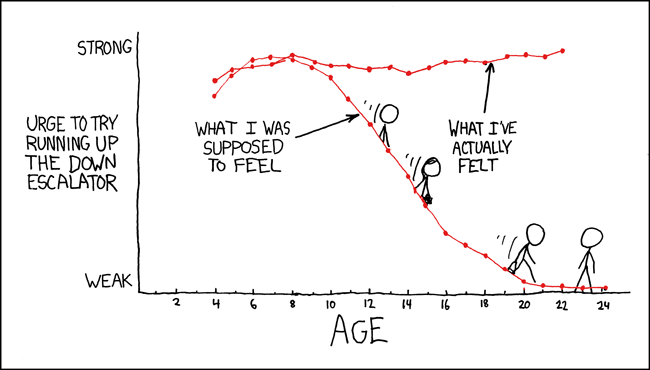
\includegraphics[width=.5\textwidth]{figures/escalators.png}}
  \end{figure}


% \begin{figure}%
%   \fbox{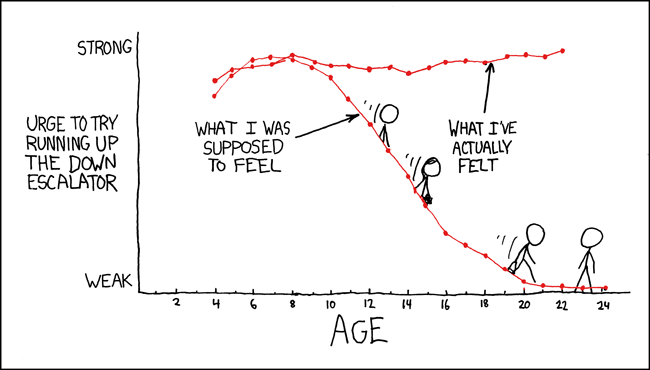
\includegraphics[width=.2\textwidth]{figures/escalators.png}}
%   \caption{An example graph illustrating the importance of captions and axis labeling. (Graphic taken from \url{https://xkcd.com/252/}.)\label{fig:xkcd}}
% \end{figure}%
                              % evaluation
\chapter{Concluding Remarks}\label{chap:conclusion}

If you wish, you may also name that section \emph{``Conclusion and Future Work''}, though it might not be a perfect choice to have a section named ``A \& B'' if it has subsections ``A'' and ``B''. Also note that you don't necessarily have to use these subsections; that also depends on how much content you have in each. (E.g., having a section header might be odd if it contains just three lines.)


\section{Conclusion}

This chapter usually summarizes the entire paper including the conclusions drawn, i.e., did the developed techniques work? Maybe add why or why not. Also note that every single scientific paper has such a section, so you can check out many examples, preferably at top-tier venues, e.g., by your supervisor(s).


\section{Future Work}

On top of that, you could discuss future work (and make clear why that is future work, i.e., by which observations did they get justified?).

Note that future work in scientific papers is often not mentioned at all or just in a very few sentences within the conclusion. That should not stop you from putting some effort in. This will (also) show the examiner(s)/supervisor(s) how well you understood the topic or how engaged you are.
                              % conclusion

\appendix
\chapter{Appendix: Explanation on Appendices}\label{chap:appendix1}

You may use appendices to provide additional information that is in principle relevant to your work, though you don't want \emph{every reader} to look at the entire material, but only those interested.

There are many cases where an appendix may make sense. For example:
\begin{itemize}
  \item You developed various variants of some algorithm, but you only describe one of them in the main body, since the different variants are not that different.
  \item You may have conducted an extensive empirical analysis, yet you don't want to provide \emph{all} results. So you focus on the most relevant results in the main body of your work to get the message across. Yet you present the remaining and complete results here for the more interested reader.
  \item You developed a model of some sort. In your work, you explained an excerpt of the model. You also used mathematical syntax for this. Here, you can (if you wish) provide the actual model as you provided it in probably some textfile. Note that you don't have to do this, as artifacts can be submitted separately. Consult your supervisor in such a case.
  \item You could also provide a list of figures and/or list of tables in here (via the commands \verb!\listoffigures! and \verb!\listoftables!, respectively). Do this only if you think that this is beneficial for your work. If you want to include it, you can of course also provide it right after the table of contents. You might want to make this dependent on how many people you think are interested in this.
\end{itemize}
                              % appendix 1
\chapter{Appendix: Explanation on Page Borders}\label{chap:appendix2}

What you find here is an explanation of why the border width keeps flipping from left to right -- which you might have spotted and wondered why that's the case.

Firstly, that is \emph{intended} and thus correct, so there is no reason to worry about this. The reason is that this document is configured as a two-sided book, which means:
\begin{compactitem}
  \item We assume the document will be printed out,
  \item that this will be done in a two-sided mode (i.e., the document will be printed on both sides of each page), and
  \item that the bookbinding will be in the middle, just like in every book.
\end{compactitem}

When you open the book, there are three borders of equal size~$n$. This however requires that even pages have a border of $n$ on their left and $\frac{n}{2}$ on their right, and odd pages have a border of $\frac{n}{2}$ on their left and $n$ on their right. This is illustrated in Figure~\ref{fig:pageBorders}.

\begin{figure}[h]
  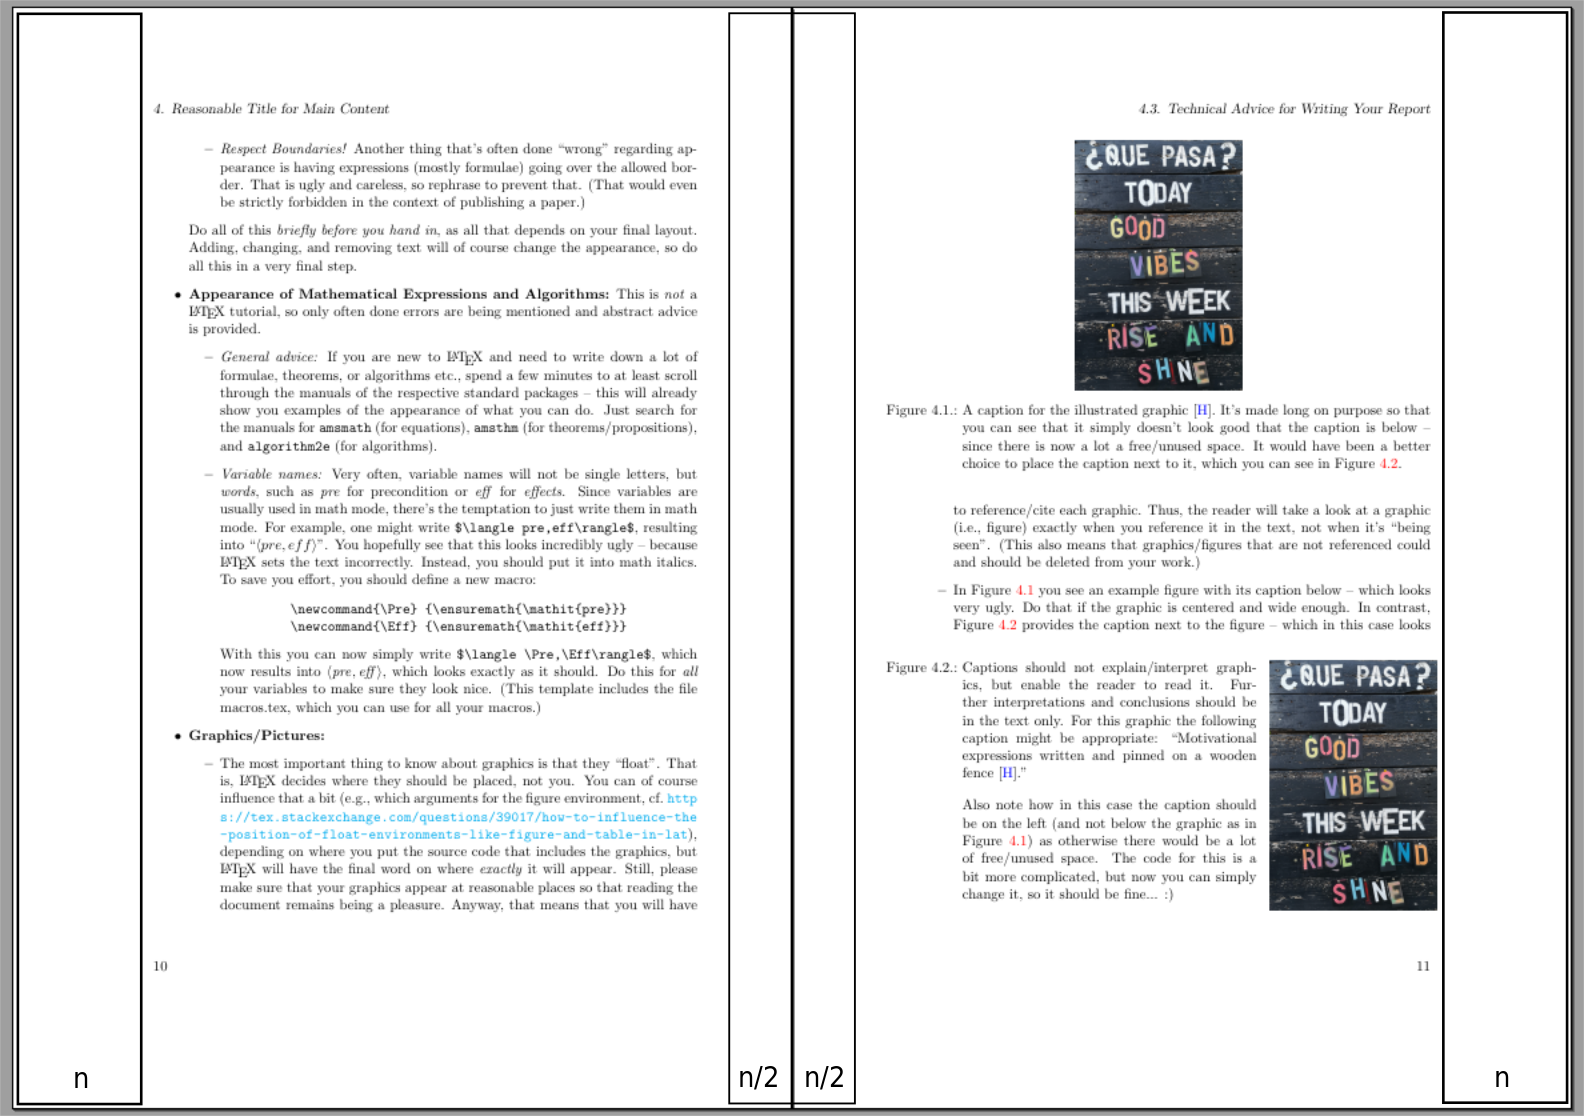
\includegraphics[width=.55\textwidth]{figures/borders--annotated}
  \caption{Illustration showing why page borders flip.\label{fig:pageBorders}}
\end{figure}%

                              % appendix 2


% literature
\bibliographystyle{anuthesis} % or plainnat or whatever
\cleardoublepage\phantomsection
% see https://tex.stackexchange.com/questions/60556/link-to-bibliography-in-the-toc-fails
\bibliography{bib}
\end{document}
